\chapter{基于反事实样本生成的图像视觉问答方法}

随着深度学习技术的发展,虽然图像视觉问答技术已经取得了长足的进步,但是目前的图像视觉问答模型往往只依赖于问题与答案之间的联系(即文本偏置)。为了缓解这一问题,最近的一些图像视觉问答模型开始引入一个辅助网络来约束目标视觉问答模型的训练,并且在标准图像视觉问答数据集VQA-CP上取得了目前最好的实验性能。然而,由于模型设计的复杂性,这类复合模型难以满足一个理想视觉问答模型应该具备的两个特点:1)视觉可解释性:在预测答案时,模型应该关注正确的视觉图像区域;2)文本敏感性:在变换问题时,模型应该感知问题的变化。因此,本章提出了一种通用的反事实样本生成机制(Counterfactual Samples Synthesizing, CSS)。CSS通过遮盖图像中的重要区域或问题中的重要单词来生成新的训练样本,然后对这些样本赋予不同的标准答案。通过使用原始训练样本和新生成训练样本一起对模型进行训练,迫使模型能够关注被遮盖的重要区域和重要单词,提升模型的视觉可解释性和文本敏感性。同样,模型的性能会被进一步提升。大量的对比实验证明CSS的有效性。值得注意的是,当对目前最好的视觉问答模型LMH~\cite{clark2019don}使用CSS机制生成样本一起训练后,模型在数据集VQA-CP v2上可以取得58.95\%的准确率,提升6.5\%。

\section{问题描述} \label{ch7:sec:introduction}
图像视觉问答(Visual Question Answering, VQA)是场景推理中一个重要的任务,也是走向真正人工智能时代至关重要的一步。图像视觉问答任务是给定一个图像和问题,模型需要根据图像内容问题回答。随着大规模视觉问答数据集的出现(如:VQA v1~\cite{antol2015vqa}和VQA v2~\cite{goyal2017making}),视觉问答任务得到了前所未有的关注。然而,由于在真实图像数据集的标注过程中不可避免地会引入偏置,目前的图像视觉问答模型往往过于依赖问题和答案之间的联系(即文本偏置)~\cite{agrawal2016analyzing,zhang2016yin,johnson2017clevr,goyal2017making}。例如,对于所有“How many”开始的问题,模型都回答“2”也可以得到较好的实验结果。为了去除之前视觉问答数据集中的偏置对视觉问答研究的影响,近期,学术界提出了一个新的数据集VQA-CP(VQA under Changing Priors)~\cite{agrawal2018don}。VQA-CP通过故意让训练集和测试集中问题和答案的分布不同,让过于依赖文本偏置的模型得到较差的实验结果。许多的视觉问答模型在VQA-CP数据集上都出现了明显的性能下降~\cite{andreas2016neural,fukui2016multimodal,yang2016stacked,anderson2018bottom}。

\begin{figure}[t]
    \centering
        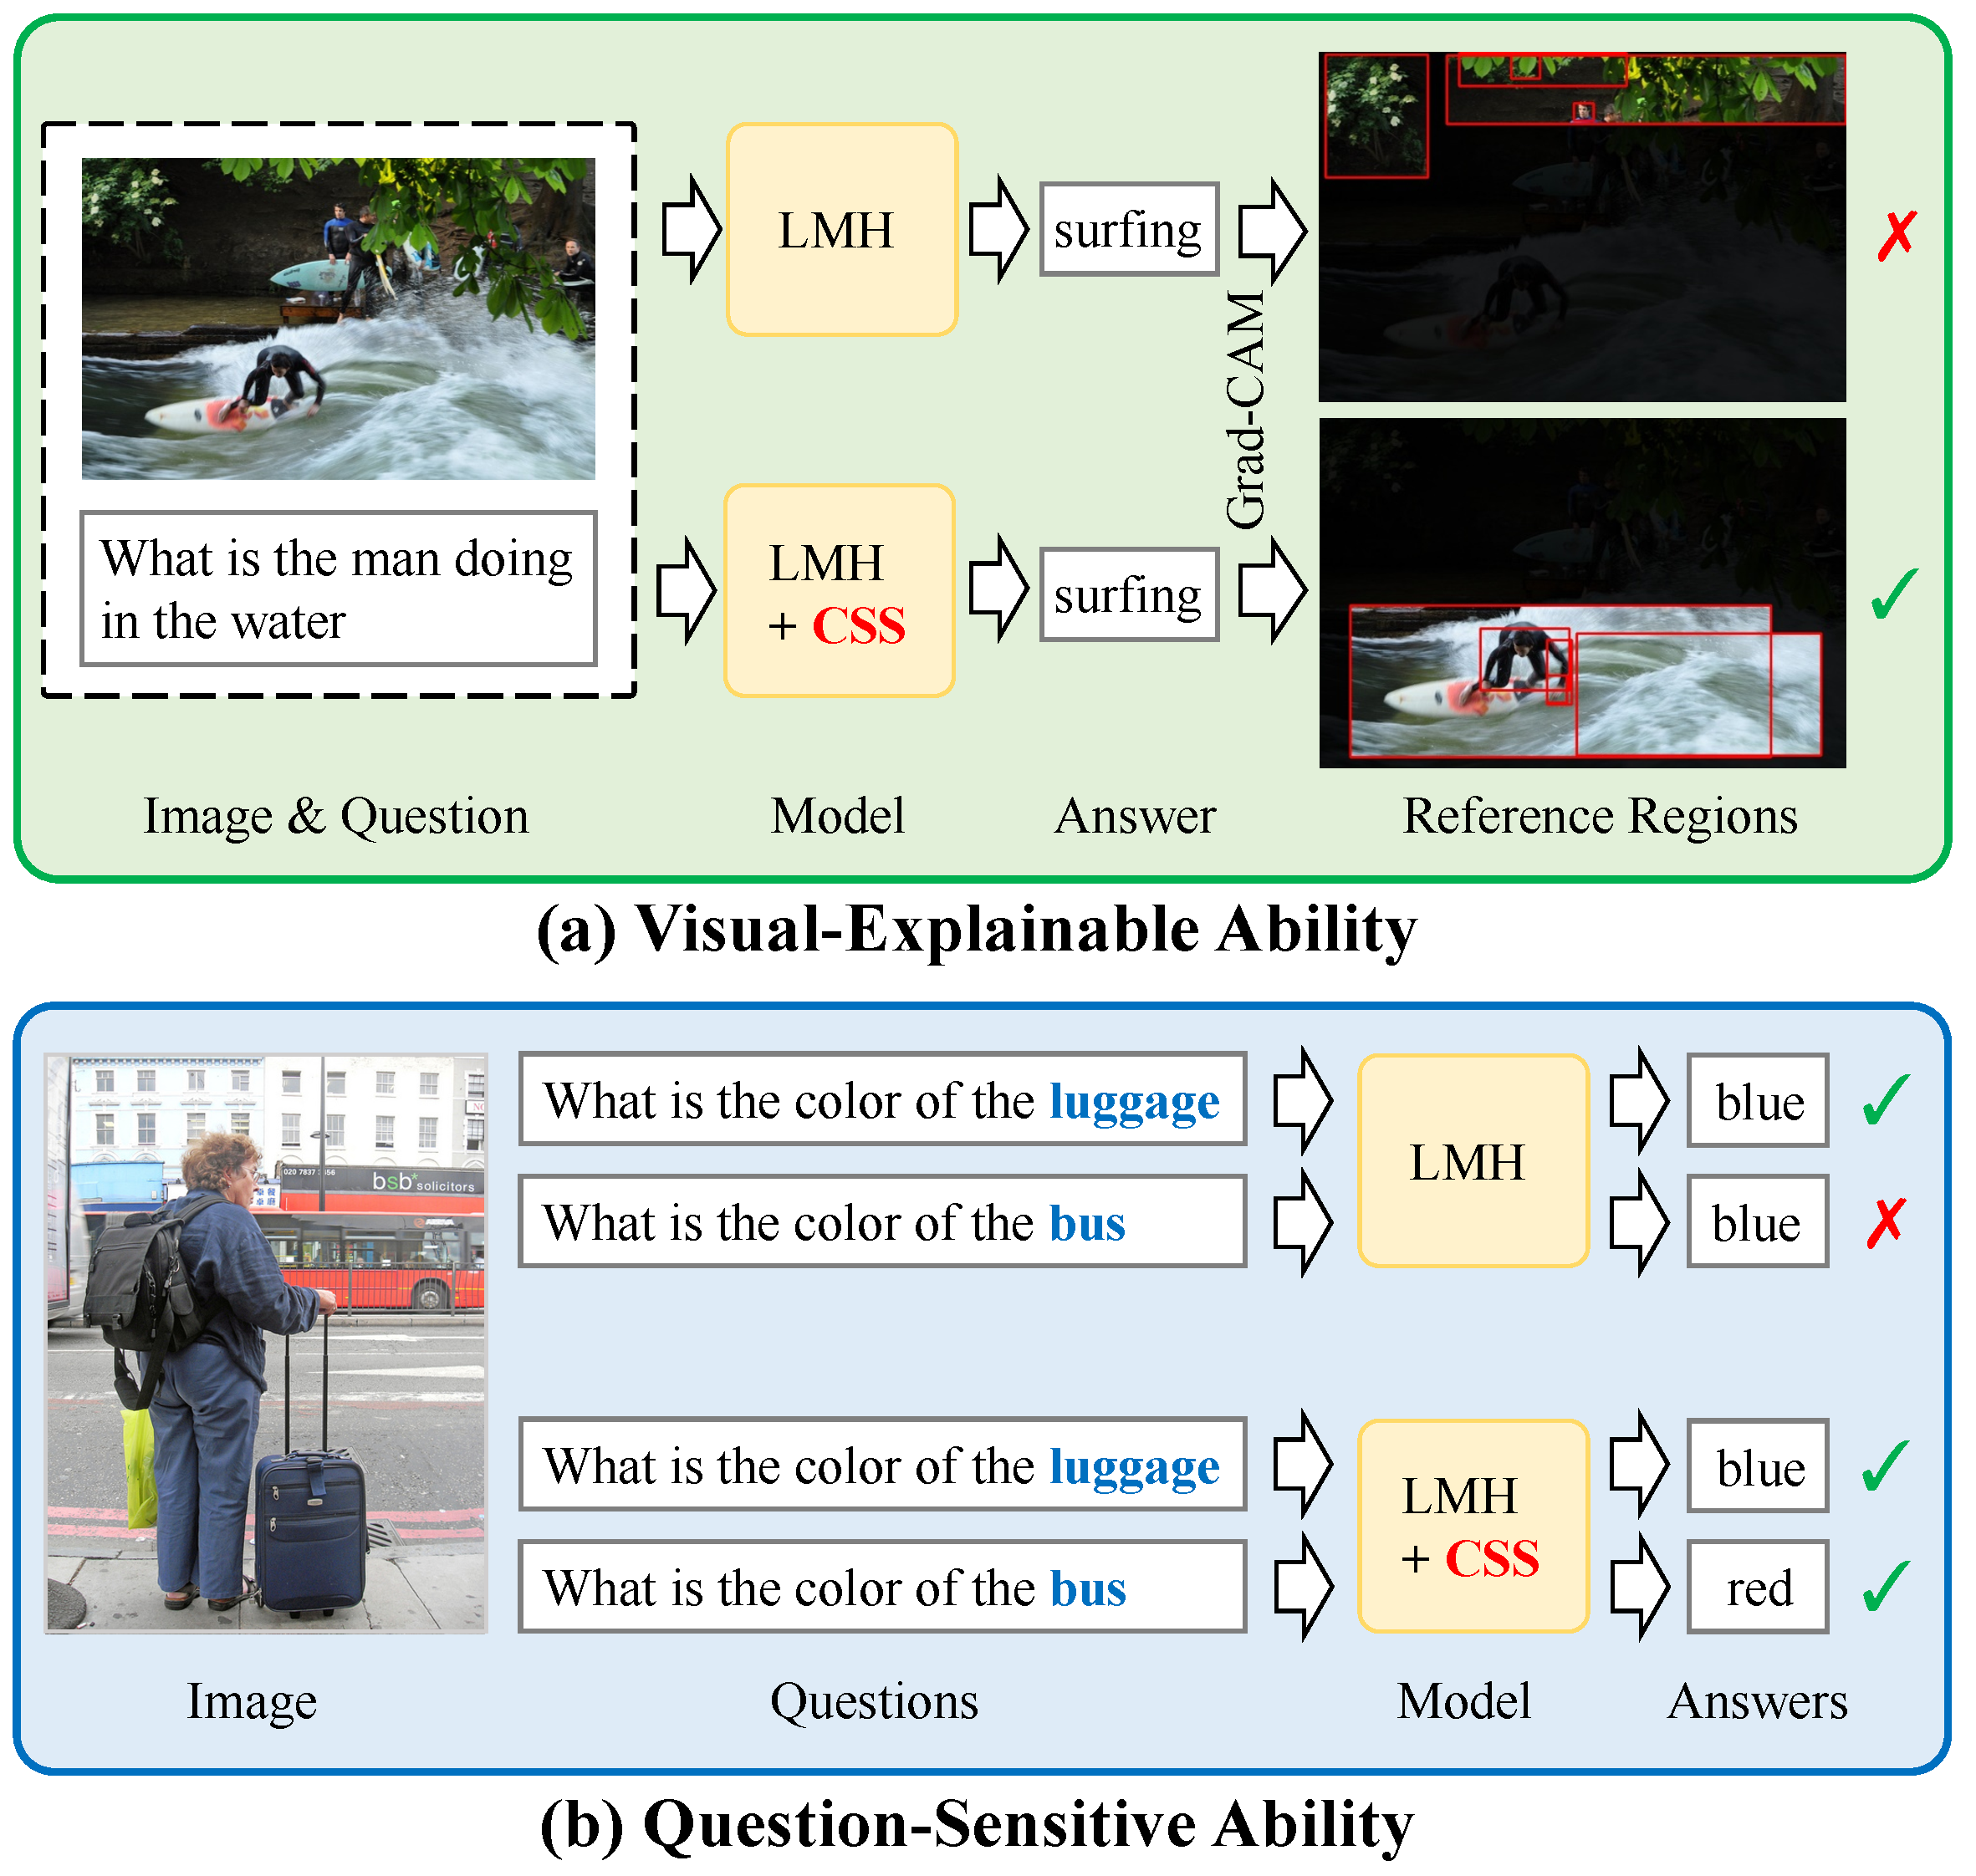
\includegraphics[width=0.8\linewidth]{chapter7/res/motivation.pdf}
    \caption{VQA模型必备的视觉可解释性和文本敏感性}
    \label{ch7:fig:motivation}
\end{figure}

目前,对于数据集VQA-CP来说,最好的解决方案都是基于复合模型的设计,即引入一个辅助网络来约束视觉问答网络的训练,其中的辅助网络只用文本(即问题语句)作为输入。具体来说,这些复合模型又可以细分为两个小类:1)基于对抗学习的方法~\cite{ramakrishnan2018overcoming,grand2019adversarial,belinkov2019don}:它们使用对抗学习~\cite{goodfellow2014generative}的方式来训练这两个网络,即减少视觉问答网络的损失函数,而增大辅助网络的损失函数。因为这两个模型共享同一个文本编码器,这类基于对抗学习的方法希望通过学习到没有偏置的文本编码向量来缓解模型过于依赖文本偏置的问题。然而,有实验表明,这类方法在计算梯度过程中引入大量噪声,造成训练过程不稳定。2)基于融合的方法~\cite{cadene2019rubi,clark2019don,mahabadi2019simple}:它们将两个网络预测答案的概率分布进行融合,然后根据融合后的概率分布计算训练梯度。这类方法的设计思想是让视觉问答网络更加关注到辅助网络无法回答的训练样本。

尽管复合模型在数据集VQA-CP上取得了最好的实验性能,但是由于目前的复合模型复杂的设计,使得这类模型难以满足一个理想视觉问答模型应该具体的两个特点:1)\textbf{视觉可解释性}:在预测答案时,模型应该关注正确的视觉图像区域~\cite{ross2017right}。如图~\ref{ch7:fig:motivation}(a)所示,尽管两个模型都可以预测出正确的答案“surfing”,但实际上两个模型是根据完全不同的视觉区域做的决策。2)\textbf{文本敏感性}:在变换问题时,模型应该感知问题的变化。如图~\ref{ch7:fig:motivation}(b)所示,当两个问题的句式结构十分接近时(如只替换“luggage”成“bus”),如果问句的意思完全不同,模型应该感知问题的差异变化,然后做出不同的预测。

\begin{figure}[t]
    \centering
        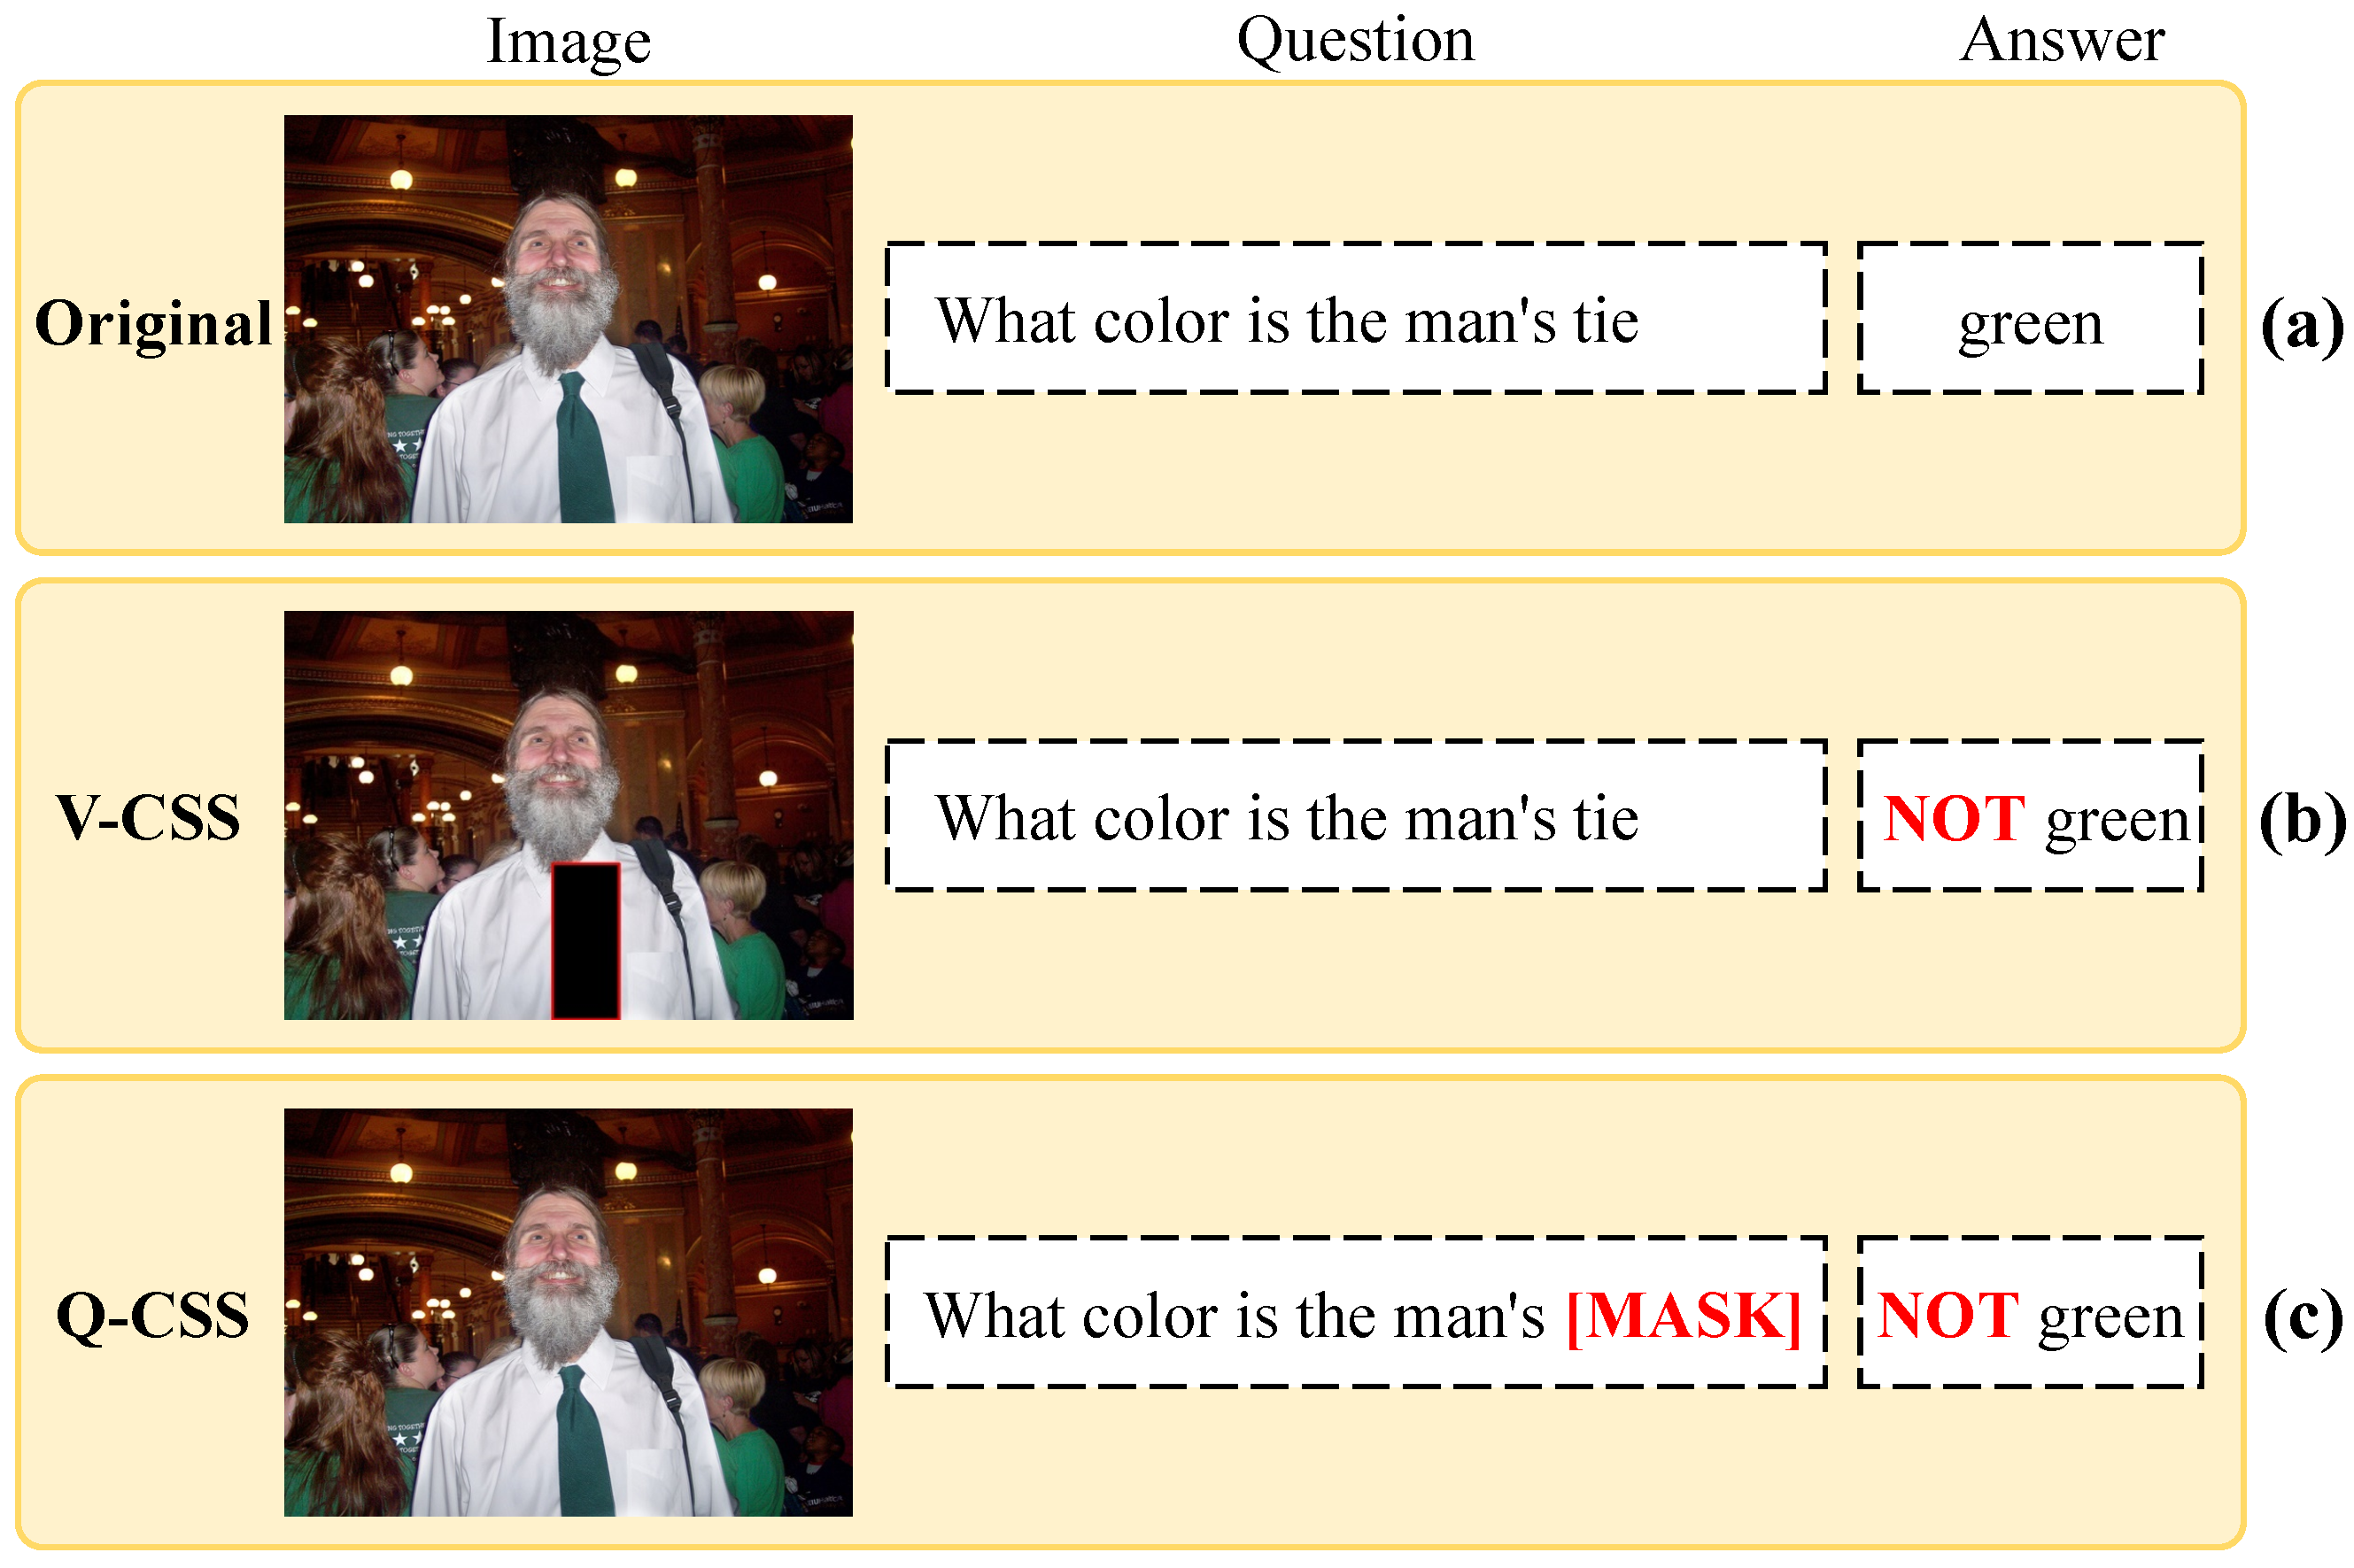
\includegraphics[width=0.8\linewidth]{chapter7/res/V-CSS_Q-CSS.pdf}
    \caption{V-CSS和Q-CSS示意图}
    \label{ch7:fig:V-CSS_Q-CSS}
\end{figure}

在本文,我们提出了一个全新的反事实样本生成机制(CSS),CSS可以“即插即用”地提升多种图像视觉问答模型的视觉可解释性和文本敏感性。如图~\ref{ch7:fig:V-CSS_Q-CSS}所示,CSS包含两种不同的样本生成机制:V-CSS和Q-CSS。对于V-CSS,我们通过遮盖图像中的重要区域,得到反事实图像。所谓的“重要区域”是指针对回答该问题非常重要的图像区域。得到的反事实图像和原始的问题就组成了一个新的图像问题对。对于Q-CSS,我们通过将原始问题中的重要单词替换成一个特定的词“[MASK]”得到反事实问题。同样,反事实问题和原始的图像也组成了一个新的图像问题对。给定一个图像问题对,一个标准的视觉问答训练样本同时还需要标准答案。为了避免大量的人工标准,我们设计了一个动态的答案生成机制,对所有新合成的图像问题对分配合理的“标准”答案(如:图~\ref{ch7:fig:V-CSS_Q-CSS}中的“not green”)。然后通过使用原始训练样本和新生成训练样本一起对模型训练,迫使模型能够关注被遮盖的重要区域和重要单词。


我们通过大量的定性实验和定量实验都验证了CSS的有效性。CSS可以无缝地用在复合模型中,不仅提升它们的视觉可解释性和文本敏感性,同时提升模型在VQA-CP上的实验性能。值得注意的是,当对目前最好的视觉问答模型LMH~\cite{clark2019don}使用CSS机制生成样本一起训练后,我们在VQA-CP v2数据集上得到58.95\%的准确率。

\section{反事实样本生成}

对于图像视觉问答任务,我们参考现有的工作将其看成一个多类别分类任务。为了不失一般性,给定一个视觉问答数据集$\mathcal{D} = \{I_i, Q_i, a_i \}^N_i$包含大量的图像$I_i \in \mathcal{I}$、问题$Q_i \in \mathcal{Q}$和答案$a_i \in \mathcal{A}$,视觉问答任务的目的在于学习一个映射函数,$f_{vqa}: \mathcal{I} \times \mathcal{Q} \rightarrow [0, 1]^{|\mathcal{A}|}$,对任意的图像问题对可以预测一个答案概率分布。为了简洁,我们在后续的表述中省略下角标$i$。

在本节,我们先介绍基本的自底向上和自顶向下模型~\cite{anderson2018bottom},以及复合模型(第~\ref{ch7:sec:preliminaries}节);其次,我们介绍CSS的具体细节(第~\ref{ch7:sec:css}节)。

\subsection{引言} \label{ch7:sec:preliminaries}

\textbf{自底向上和自顶向下模型}(Bottom-Up Top-Down, UpDn):对于每张图像$I$,UpDn模型使用图像编码器$e_v$将图像编码成一系列物体特征:$\bm{V} = \{\bm{v}_1, ..., \bm{v}_{n_v}\}$,其中$\bm{v}_i$表示第$i$个物体特征。对于每个问题$Q$,UpDn模型使用问题编码器$e_q$编码成一系列单词特征:$\bm{Q} = \{\bm{w}_1, ..., \bm{w}_{n_q}\}$,其中$\bm{w}_j$表示第$j$个单词的特征。然后特征$\bm{V}$和$\bm{Q}$都输入到模型$f_{vqa}$中来预测答案概率分布:
\begin{equation} \label{ch7:eq:p_vqa}
    P_{vqa}(\bm{a}|I, Q) = f_{vqa}(\bm{V}, \bm{Q})
\end{equation}
其中,模型$f_{vqa}$通常包含一个注意力机制,然后利用交叉熵作为损失函数对模型进行优化。

\textbf{复合模型}:由前文提到(第~\ref{ch7:sec:introduction}节)提到,复合模型主要细分为两小类:基于对抗学习的方法和基于融合的方法。因为基于对抗学习的方法~\cite{ramakrishnan2018overcoming,grand2019adversarial,belinkov2019don}训练过程不稳定,在本节,我们只介绍基于融合的方法~\cite{cadene2019rubi,clark2019don,mahabadi2019simple}。如算法~\ref{ch7:alg:VQA},它们通过引入辅助网络$f_q$,只利用问题$\bm{Q}$做为输入:
\begin{equation}
P_{q}(\bm{a}|Q) = f_{q}(\bm{Q})
\end{equation}
然后,它们通过一个融合函数$M$将两个网络的概率分布进行融合:
\begin{equation}
\hat{P}_{vqa}(\bm{a}|I, Q) = M(P_{vqa}(\bm{a}|I, Q), P_{q}(\bm{a}|Q))
\end{equation}
在训练阶段,直接基于融合后的答案分布$\hat{P}_{vqa}(\bm{a})$计算交叉熵损失,然后计算梯度优化$f_{vqa}$和$f_q$。在测试阶段,只使用模型$f_{vqa}$。

\begin{algorithm}[t]
    \caption{复合模型(基于融合的方法)}\label{ch7:alg:VQA}
    \begin{algorithmic}[1]
        \Function {$\mathcal{\textcolor{blue}{VQA}}$}{$I, Q, a, cond$}
        \State $ \bm{V} \leftarrow e_v(I) $
        \State $ \bm{Q} \leftarrow e_q(Q) $
        \State $ P_{vqa}(\bm{a}) \leftarrow f_{vqa}(\bm{V}, \bm{Q}) $
        \State $ P_{q}(\bm{a}) \leftarrow f_{q}(\bm{Q})$      \Comment{辅助模型}
        \State $ \hat{P}_{vqa}(\bm{a}) \leftarrow M(P_{vqa}(\bm{a}), P_{q}(\bm{a}))  $
        \State $ Loss \leftarrow \text{XE}(\hat{P}_{vqa}(\bm{a}), a)$ \Comment{参数更新}
        \If{$cond$}
        \State \textbf{return} $\bm{V}, \bm{Q}, P_{vqa}(\bm{a})$
        \EndIf 
        \EndFunction
    \end{algorithmic}
\end{algorithm}

\subsection{反事实样本生成} \label{ch7:sec:css}
整个反事实样本生成(CSS)算法的流程展示在算法~\ref{ch7:alg:CSS}。具体来说,对于给定的一个视觉问答模型(即$\mathcal{VQA}$)和训练样本$(I, Q, a)$,CSS主要包含三个步骤:

\begin{asparaenum}
\item 用原始的训练样本对$\mathcal{\textcolor{blue}{VQA}}$模型进行训练;

\item 用V-CSS生成反事实样本$(I^-, Q, a^-)$或用Q-CSS生成反事实样本$(I, Q^-, a^-)$;

\item 用新生成的反事实样本对$\mathcal{\textcolor{blue}{VQA}}$模型进行训练。
\end{asparaenum}

在接下来,我们先详细介绍两种反事实样本生成机制:V-CSS和Q-CSS。如算法~\ref{ch7:alg:CSS}所示,对于每个训练样本,我们只使用特定的一种样本生成机制,其中$\delta$是一个超参数来权衡两种生成机制的比例。


\begin{algorithm}[tbp]
    \caption{反事实样本生成}\label{ch7:alg:CSS}
    \begin{algorithmic}[1]
        \Function {$\mathcal{CSS}$}{$I, Q, a$}
        \State $ \bm{V}, \bm{Q}, P_{vqa}(\bm{a}) \leftarrow \mathcal{\textcolor{blue}{VQA}}(I, Q, a, \text{True})$
        \State $ cond \sim U[0, 1]$
        \If {$cond \geq \delta $}  \Comment{执行V-CSS}
            \State $ \mathcal{I} \leftarrow  \textsc{IO\_Sel}(I, Q) $
            \State $ s(a, \bm{v}_i) \leftarrow \mathcal{S}(P_{vqa}(a), \bm{v}_i)$
            \State $ I^+, I^- \leftarrow \textsc{CO\_Sel}(\mathcal{I}, \{s(a, \bm{v}_i) \}) $
            \State $ a^- \leftarrow \textsc{DA\_Ass}(I^+, Q, \mathcal{VQA}, a) $
            \State $ \mathcal{\textcolor{blue}{VQA}}(I^-, Q, a^-, \text{False})$
        \Else \Comment{执行Q-CSS}
            \State $ s(a, \bm{w}_i) \leftarrow \mathcal{S}(P_{vqa}(a), \bm{w}_i) $
            \State $ Q^+, Q^- \leftarrow \textsc{CW\_Sel}(\{s(a, \bm{w}_i)\})$
            \State $ a^- \leftarrow \textsc{DA\_Ass}(I, Q^+, \mathcal{VQA}, a) $
            \State $ \mathcal{\textcolor{blue}{VQA}}(I, Q^-, a^-, \text{False})$
        \EndIf
        \EndFunction
    \end{algorithmic}
\end{algorithm}


\textbf{V-CSS}:我们将按照程序执行顺序陆续介绍V-CSS的主要步骤(即算法~\ref{ch7:alg:CSS}中第5行-第8行):初始物体选择(\textsc{IO\_Sel})、物体局部贡献计算、重要物体选择(\textsc{CO\_Sel})和动态答案生成(\textsc{DA\_Ass}):

初始物体选择(\textsc{IO\_Sel}):通常给定一个图像问题对$(Q, a)$,图像中只有部分物体与当前问题有关。为了缩小后续重要物体选择的范围,我们首先构建一个小的物体集$\mathcal{I}$,使得物体集$\mathcal{I}$中的物体都可能对回答正确问题有帮助。因为缺乏人工的标注,我们参考Wu等人~\cite{wu2019self}先提取与问答语句十分相关的物体。具体来说,我们先用spaCy POS tagger~\cite{honnibal2017spacy}提取问答中的所有名词,然后利用所有名词和类别的GloVe编码~\cite{pennington2014glove}计算余弦相似度,其中相似度记为$\mathcal{SIM}$。之后根据$\mathcal{SIM}$选择分数最高的$|\mathcal{I}|$个物体作为$\mathcal{I}$。

物体局部贡献计算:当得到物体集$\mathcal{I}$之后,我们开始计算每个物体对最终的正确答案的局部贡献。我们参考现有的工作~\cite{jain2019attention,selvaraju2019taking,wu2019self},同样使用修改的Grad-CAM~\cite{selvaraju2017grad}算法来计算局部贡献。对于第$i$个物体来说,它对正确答案$a$的贡献为:
\begin{equation} \label{ch7:eq:eq_4}
s(a, \bm{v}_i) = \mathcal{S}(P_{vqa}(a), \bm{v}_i) \coloneqq (\nabla_{\bm{v}_i} P_{vqa}(a))^T\mathbf{1}
\end{equation}
其中$P_{vqa}(a)$表示对正确答案$a$的预测概率,$\bm{v}_i$表示第$i$个物体特征,$\mathbf{1}$表示向量所有元素都为1。显然,如果分数$s(a, \bm{v}_i)$越高,物体特征$\bm{v}_i$对正确答案$a$的贡献也越大。

重要物体选择(\textsc{CO\_Sel}):在对物体集$\mathcal{I}$中每个物体计算局部贡献$s(a, \bm{v}_i)$之后,我们将分数最大的前K个物体当成重要的物体,即$I^+$。对于每张图像,K是满足公式~\eqref{ch7:eq:eq_5}最小的数:
\begin{equation} \label{ch7:eq:eq_5}
\sum_{\bm{v}_i \in I^+} \exp(s(a, \bm{v}_i)) / \sum_{\bm{v}_j \in \mathcal{I}} \exp(s(a, \bm{v}_j))  > \eta
\end{equation}
其中$\eta$是一个常数,所有的实验中我们将$\eta$设定为0.65。然后反事实图像就是物体集$I^+$在所有物体$I$中的补集,即$I^- = I \backslash I^+$。图~\ref{ch7:fig:IQ+-}展示了一个$I$、$I^+$和$I^-$的示例。

动态答案生成(\textsc{DA\_Ass}):给定反事实图像$I^-$和原始问题$Q$,我们可以组成一个新的图像问题对($I^-, Q$)。作为训练样本,新的图像问题对同样需要分配标准答案。为了减少人工标准的成本,我们设计了一种动态的答案生成机制,预测一个标准答案$a^-$。动态答案生成机制的细节在算法~\ref{ch7:alg:daass}。具体来说,我们将另一个图像问题对($I^+, Q$)输入到视觉问答模型$\mathcal{VQA}$中,然后得到预测的答案概率分布$P^+_{vqa}(\bm{a})$。根据概率$P^+_{vqa}(\bm{a})$,我们选取前N个答案作为$a^+$,然后定义$ a^- \coloneqq \{a_i | a_i \in a, a_i \notin a^+ \}$。极端情况下,如果模型对于图像问题对($I^+, Q$)可以回答全部的正确答案,即$a \subset a^+$,则$a^-$为空集$\emptyset$。

\begin{algorithm}[tbp]
    \caption{动态答案生成}\label{ch7:alg:daass}
    \begin{algorithmic}[1]
        \Function {$\textsc{DA\_Ass}$}{$I^+, Q^+, \mathcal{VQA}, a$}
        \State  $\mathcal{VQA}$.eval() \Comment{不更新参数}
        \State  $ \_, \_, P_{vqa}^+(\bm{a}) \leftarrow \mathcal{VQA}(I^+, Q^+, a, \text{True}) $
        \State $ a^+ \leftarrow \text{top-N}(\text{argsort}_{a_i \in \mathcal{A}}(P_{vqa}^+(a_i)))$
        \State $ a^- \coloneqq \{a_i | a_i \in a, a_i \notin a^+ \} $ \Comment{$a$是标准答案集}
        \State \textbf{return} $a^-$
        \EndFunction
    \end{algorithmic}
\end{algorithm}

\begin{figure}[t]
    \centering
        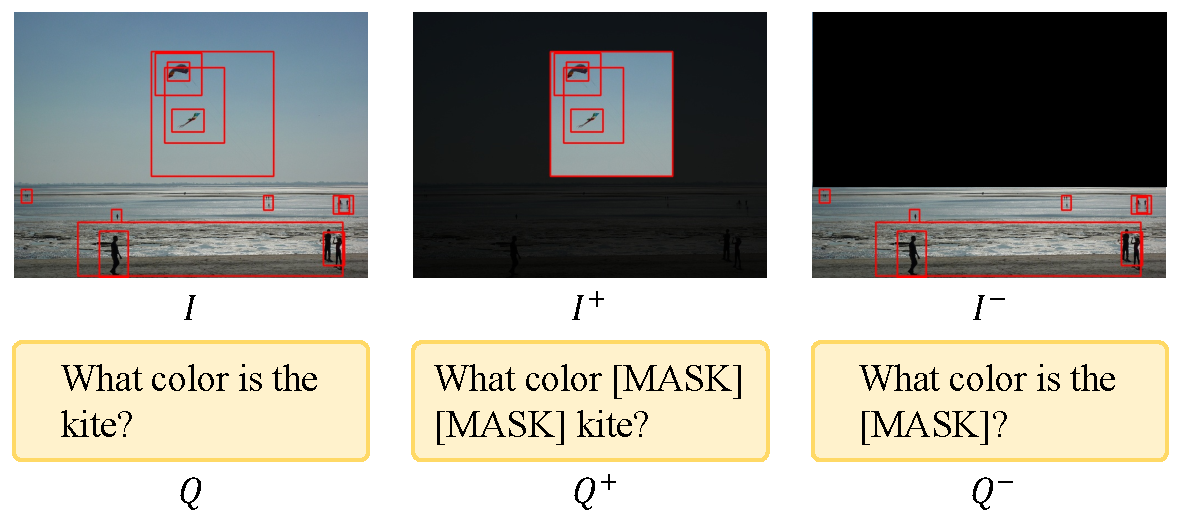
\includegraphics[width=0.8\linewidth]{chapter7/res/IQ+-.pdf}
    \caption{$I^+$、$I^-$、$Q^+$和$Q^-$的示例图}
    \label{ch7:fig:IQ+-}
\end{figure}

\textbf{Q-CSS}: 对于Q-CSS,主要的步骤和V-CSS非常接近,除了没有初始物体选择(即\textsc{IO\_Sel})。按照算法执行的顺序(算法~\ref{ch7:alg:CSS}第11行至第14行),Q-CSS主要包含三步:单词局部贡献计算、重要单词选择(\textsc{CW\_Sel})和动态答案生成(\textsc{DA\_Ass})。

单词局部贡献计算:与V-CSS(公式~\eqref{ch7:eq:eq_4})相似,对于第$i$个单词来说,它对正确答案$a$的贡献为:
\begin{equation} \label{ch7:eq:eq_6}
s(a, \bm{w}_i) = \mathcal{S}(P_{vqa}(a), \bm{w}_i) \coloneqq (\nabla_{\bm{w}_i} P_{vqa}(a))^T\mathbf{1}
\end{equation}

重要单词选择(\textsc{CW\_Sel}):对于这步,我们首先提取每个问题$Q$的问题类别前缀,这些前缀直接使用数据集VQA-CP默认的问题类别前缀。然后对剩余的单词选择贡献最高的K个单词作为重要单词。反事实问句$Q^-$就是将问句$Q$中的重要单词替换成一个特殊字符“[MASK]”。图~\ref{ch7:fig:IQ+-}展示了一个$Q$、$Q^+$和$Q^-$的示例。

动态答案生成(\textsc{DA\_Ass}):这个动态答案生成步骤和V-CSS的完全相同,即算法~\ref{ch7:alg:daass}。对于Q-CSS,\textsc{DA\_Ass}的输入是图像问题对$(I, Q^+)$。


\section{实验设置与性能对比}

我们主要在数据集VQA-CP~\cite{agrawal2018don}的测试集上对模型性能进行验证。为了实验比较的完整性,我们同样在VQA v2~\cite{goyal2017making}的验证集上进行测试。关于模型的准确率,我们使用通用的VQA准确率计算方式~\cite{antol2015vqa}。为了实验比较的公平性,所有的实验都采取与UpDn模型~\cite{anderson2018bottom}相同的数据预处理。

\subsection{CSS对视觉问答的性能分析}

\textbf{CSS机制中不同超参数选择的影响}:我们通过大量的对比实验来分析V-CSS和Q-CSS中不同超参数对模型性能的影响。具体来说,所有的实验都是基于模型LMH~\cite{clark2019don}。实验结果展示在图~\ref{ch7:fig:ablative_studies}中。

V-CSS中初始物体选择$\mathcal{I}$的大小:不同$\mathcal{I}$的大小对实验性能的影响如图~\ref{ch7:fig:ablative_studies}(a)所示。随着$\mathcal{I}$的增加,模型的性能逐渐降低。

V-CSS中重要物体选择的数量:不同重要物体选择的数量对实验性能的影响如图~\ref{ch7:fig:ablative_studies}(a)所示。我们比较了动态选择K(公式~\ref{ch7:eq:eq_5})和预先固定一些常数(如:1、3或5)。从实验结果可知,动态选择K个中国物体可以得到最佳性能。

Q-CSS中重要单词选择的数量:不同重要单词选择的数量对实验性能的影响如图~\ref{ch7:fig:ablative_studies}(b)所示。从实验结果可知,只选择一个单词作为重要单词性能最好。

V-CSS和Q-CSS的比例$\delta$:不同$\delta$对实验性能的影响如图~\ref{ch7:fig:ablative_studies}(c)所示。从实验结果可知,$\delta = 0.5$性能最好。


\begin{figure*}[t]
    \centering
    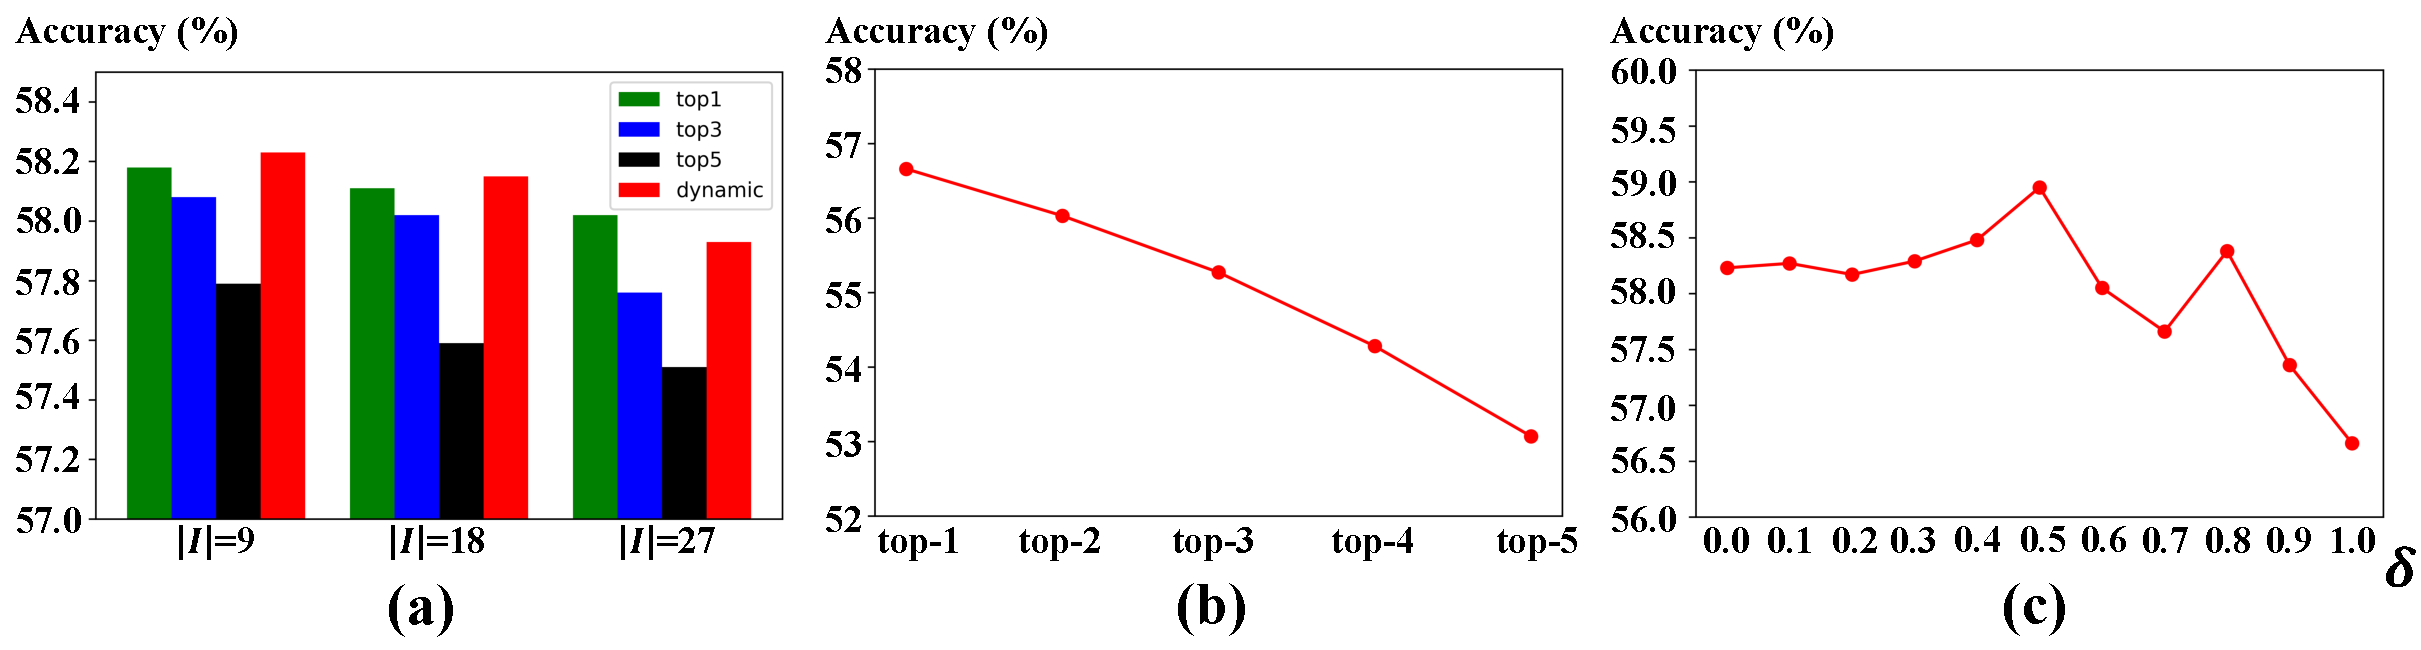
\includegraphics[width=\linewidth]{chapter7/res/ablative_studies.pdf}
    \caption{\textbf{消融实验}:不同超参数对V-CSS和Q-CSS性能的影响}
    \label{ch7:fig:ablative_studies}
\end{figure*}


\textbf{CSS机制对模型的通用性}:因为本章提出的CSS训练机制可以适用于不同的VQA模型中。为了验证CSS对不同模型结构性能的有效性,我们将CSS机制应用于多种VQA模型中:\textbf{UpDn}~\cite{anderson2018bottom}、\textbf{PoE} (Product of Experts)~\cite{clark2019don,mahabadi2019simple}、\textbf{RUBi}~\cite{cadene2019rubi}、\textbf{LMH}~\cite{clark2019don}。特别地,模型PoE、RUBi、LMH属于复合模型。所有的实验结果展示在表~\ref{ch7:tab:boost_models},其中$^\dagger$表示我们的重现结果。

和不同VQA结构的基准模型对比,CSS同时可以提升不同模型的性能。由于对于复合模型来说,性能的提升更加明显(例如:在LMH和PoE模型中分别提升6.5\%和9.79\%)。通常情况下,同时使用两种CSS机制(即V-CSS和Q-CSS)可以得到最佳性能。


%%%%%% Boost Ensemble-based Models  %%%%%%%%%%%%%%%
\begin{table}[tbp]
    \begin{center}
        \scalebox{0.90}{
            \begin{tabular}{|l | l | l | c c c c|}
                \hline
                & & Model & All & Y/N & Num & Other  \\
                \hline
                \parbox[t]{2mm}{\multirow{5}{*}{\rotatebox[origin=c]{90}{Plain Models}}} & \multirow{5}{*}{UpDn~\cite{anderson2018bottom}} & Baseline & 39.74 & 42.27 & 11.93  & 46.05 \\
                & & Baseline$^\dagger$ & 39.68 & 41.93 & 12.68 & 45.91 \\
                & & ~+Q-CSS & 40.05 & 42.16 & 12.30 & 46.56 \\
                & & ~+V-CSS & 40.98 & 43.12 & 12.28 & 46.86 \\
                & & ~+$\mathcal{CSS}$ & \textbf{41.16} & \textbf{43.96} & \textbf{12.78} & \textbf{47.48} \\
                \hline
                \parbox[t]{2mm}{\multirow{15}{*}{\rotatebox[origin=c]{90}{Ensemble-Based Models}}} & \multirow{5}{*}{PoE~\cite{clark2019don, mahabadi2019simple}} & Baseline & 39.93 & -- & --  & -- \\
                & & Baseline$^\dagger$ & 39.86 & 41.96 & 12.59 & 46.25 \\
                & & ~+Q-CSS & 40.73 & 42.99 & 12.49 & \textbf{47.28} \\
                & & ~+V-CSS & \textbf{49.65} & \textbf{74.98} & \textbf{16.41} & 45.50 \\
                & & ~+$\mathcal{CSS}$& 48.32 & 70.44 & 13.84 & 46.20 \\
                \cline{2-7}
                & \multirow{5}{*}{RUBi~\cite{cadene2019rubi}} & Baseline & 44.23 & -- & --  & -- \\
                & & Baseline$^\dagger$ & 45.23 & 64.85 & 11.83 & 44.11 \\
                & & ~+Q-CSS & 46.31 & \textbf{68.70} & \textbf{12.15} & 43.95 \\
                & & ~+V-CSS & 46.00 & 62.08 & 11.84 & \textbf{46.95} \\
                & & ~+$\mathcal{CSS}$ & \textbf{46.67} & 67.26 & 11.62 & 45.13 \\
                \cline{2-7}
                & \multirow{5}{*}{LMH~\cite{clark2019don}} & Baseline & 52.05 & -- & --  & -- \\
                & & Baseline$^\dagger$ & 52.45 & 69.81 & 44.46 & 45.54 \\
                & & ~+Q-CSS & 56.66 & 80.82 & 45.83 & 46.98 \\
                & & ~+V-CSS & 58.23 & 80.53 & \textbf{52.48} & 48.13 \\
                & & ~+$\mathcal{CSS}$ & \textbf{58.95} & \textbf{84.37} & 49.42 & \textbf{48.21} \\
                \hline
            \end{tabular}
        } % scale box
    \end{center}
    \caption{CSS机制对不同VQA模型的提升作用}
    \label{ch7:tab:boost_models}
\end{table}

\subsection{视觉问题方法性能对比}

\textbf{数据集VQA-CP v2和VQA v2上性能对比}:
我们将CSS机制应用于模型LMH~\cite{clark2019don}中,然后标记为\textbf{LMH-CSS}。我们将LMH-CSS与其他目前性能最好的视觉问答模型在数据集VQA-CP v2和VQA v2上进行性能对比。根据模型的骨干网络不同,我们可以将模型分为两大类:1)\textbf{AReg}~\cite{ramakrishnan2018overcoming}、\textbf{MuRel}~\cite{cadene2019murel}、\textbf{GRL}~\cite{grand2019adversarial}、\textbf{RUBi}~\cite{cadene2019rubi}、\textbf{SCR}~\cite{wu2019self}、\textbf{LMH}~\cite{clark2019don}和\textbf{HINT}~\cite{selvaraju2019taking}。这些模型都是将\textbf{UpDn}~\cite{anderson2018bottom}作为骨干网络。2) \textbf{HAN}~\cite{malinowski2018learning}、\textbf{GVQA}~\cite{agrawal2018don}、\textbf{ReGAT}~\cite{li2019relation}、\textbf{NSM}~\cite{hudson2019learning}。这些模型都是使用其他不同的骨干网络。例如:模型BLOCK~\cite{ben2019block}、BAN~\cite{kim2018bilinear} 等。特别地,AReg、GRL、RUBi和LMH都是复合模型。

所有的实验结果都展示在表~\ref{ch7:tab:SOTA_v2}中。当在数据集VQA-CP v2上进行训练和测试时,LMH-CSS在所有的问题类别上都可以达到目前最好实验性能。特别地,CSS可以大幅提升LMH模型6.5\%的准确率(58.95\% vs. 52.45\%)。当在数据集VQA v2上进行训练和测试时,CSS只造成了细微了性能下降(1.74\%)。为了对比的完整性,我们比较了两个不同数据集中性能的差异。相比于之前的模型往往存在较大的性能差异(例如:UpDn模型中存在23.74\%、LMH模型中存在9.19\%),LMH-CSS可以显著地将性能差异减少至0.96\%。这也间接说明CSS可以显著缓解模型对文本偏置的依赖。


%%%%%%%%%%%%% STOA on VQA-CP v2 %%%%%%%%%%%%%%%%
\begin{table*}
    \begin{center}
        \scalebox{0.85}{
            \begin{tabular}{| l | c c c c | c c c c| c |}
                \hline
                \multirow{2}{*}{Model}  & \multicolumn{4}{c|}{VQA-CP v2 test $\uparrow$} & \multicolumn{4}{c|}{VQA v2 val $\uparrow$} & Gap$\Delta$$\downarrow$ \\
                & All & Yes/No & Num & Other & All & Yes/No & Num & Other & All \\
                \hline
                HAN~\cite{malinowski2018learning} & 28.65 & 52.25 & 13.79 & 20.33 & -- & -- & -- & -- & --  \\
                GVQA~\cite{agrawal2018don} & 31.30 & 57.99 & 13.68 & 22.14 & 48.24 & 72.03 & 31.17 & 34.65 & 16.94 \\
                ReGAT~\cite{li2019relation} & 40.42 & -- & -- & -- & 67.18 & -- & -- & -- & 26.76 \\
                RUBi~\cite{cadene2019rubi} & 47.11 & 68.65 & 20.28 & 43.18 & 61.16 & -- & -- & -- & 14.05  \\ 
                NSM~\cite{hudson2019learning} & 45.80 & -- & -- & -- & -- & -- & -- & -- & -- \\
                \cline{1-1}
                UpDn~\cite{anderson2018bottom} & 39.74 & 42.27 & 11.93 & 46.05 & 63.48 & 81.18 & 42.14 & 55.66 & 23.74 \\
                ~~~~+AReg$^\dagger$~\cite{ramakrishnan2018overcoming} & 41.17 & 65.49 & 15.48 & 35.48 & 62.75 & 79.84 & 42.35 & 55.16 & 21.58 \\
                ~~~~+MuRel~\cite{cadene2019murel} & 39.54 & 42.85 & 13.17 & 45.04 & -- & -- & -- & --  & -- \\
                ~~~~+GRL$^\dagger$~\cite{grand2019adversarial} & 42.33 & 59.74 & 14.78 & 40.76 & 51.92 & -- & -- & -- & 9.59 \\
                ~~~~+RUBi$^\dagger$$^*$~\cite{cadene2019rubi} & 45.23 & 64.85 & 11.83 & 44.11 & 50.56 & 49.45 & 41.02 & 53.95 & 5.33  \\
                ~~~~+SCR~\cite{wu2019self} & 48.47 & 70.41 & 10.42 & 47.29 & 62.30 & 77.40 & 40.90 & 56.50 & 13.83  \\
                ~~~~+LMH$^\dagger$$^*$~\cite{clark2019don} & 52.45 & 69.81 & 44.46 & 45.54 & 61.64 & 77.85 & 40.03 & 55.04 & 9.19  \\
                ~~~~+\textbf{LMH-CSS} & \textbf{58.95} & \textbf{84.37} & \textbf{49.42} & \textbf{48.21} & 59.91 & 73.25 & 39.77 & 55.11 & \textbf{0.96}  \\
                \hline\hline
                ~~~~+HINT+HAT~\cite{selvaraju2019taking} & 47.70 & 70.04 & 10.68 & 46.31 & 62.35 & 80.49 & 41.75 & 54.01 & 14.65 \\
                ~~~~+SCR+HAT~\cite{wu2019self} & 49.17 & 71.55 & 10.72 & 47.49 & 62.20 & 78.90 & 41.40 & 54.30 & 13.03  \\
                ~~~~+SCR+VQA-X~\cite{wu2019self} & 49.45 & 72.36 & 10.93 & 48.02 & 62.20 & 78.80 & 41.60 & 54.40 & 12.75  \\
                \hline
            \end{tabular}
        } % scale box
    \end{center}
    \caption{不同模型在VQA-CP v2和VQA v2数据集上的性能对比} % \footnotemark
    \label{ch7:tab:SOTA_v2}
\end{table*}
%%%%%%%%%%%%%%%%%%%%%%%%%%%%%%%%%%

\textbf{数据集VQA-CP v1上性能对比}:我们同时将LMH-CSS于目前最好的视觉问答模型在数据集VQA-CP v1上进行性能对比。同样,根据骨干网络,我们将这些模型分为:1) \textbf{GVQA}。它是使用SAN~\cite{yang2016stacked}模型作为骨干网络。2)\textbf{AReg}、\textbf{GRL}、\textbf{RUBi}和\textbf{LMH}。这些模型都是使用UpDn模型作为骨干网络。

所有的实验结果都展示在表~\ref{ch7:tab:SOTA_v1}中。通过和其他模型对比,LMH-CSS在数据集VQA-CP v1上可以达到目前最好的实验性能。特别地,CSS可以提升LMH模型5.68\%的准确率(60.95\%相比于55.27\%)。

%%%%%%%%%%%%% STOA on VQA-CP v1 %%%%%%%%%%%%%%%%
\begin{table}[tbp]
    \begin{center}
        \scalebox{0.9}{
            \begin{tabular}{| l | c c c c|}
                \hline
                Model & All & Yes/No & Num & Other  \\
                \hline
                GVQA~\cite{agrawal2018don}  & 39.23 & 64.72 & 11.87 & 24.86 \\
                UpDn~\cite{anderson2018bottom} & 39.74 & 42.27 & 11.93 & \textbf{46.05} \\
                ~~~+AReg$^\dagger$~\cite{ramakrishnan2018overcoming} & 41.17 & 65.49 & 15.48 & 35.48 \\
                ~~~+GRL$^\dagger$~\cite{grand2019adversarial} &  45.69 & 77.64 & 13.21 & 26.97 \\
                ~~~+RUBi$^\dagger$$^*$~\cite{cadene2019rubi} & 50.90 & 80.83 & 13.84 & 36.02 \\
                ~~~+LMH$^\dagger$$^*$~\cite{clark2019don} & 55.27 & 76.47 & 26.66 & 45.68 \\
                \hline
                ~~~+\textbf{LMH-CSS} & \textbf{60.95} & \textbf{85.60} & \textbf{40.57} & 44.62  \\
                \hline
            \end{tabular}
        } % scale box
    \end{center}
    \caption{不同模型在VQA-CP v1数据集上的性能对比}
    \label{ch7:tab:SOTA_v1}
\end{table}
%%%%%%%%%%%%%%%%%%%%%%%%%%%%%%%%%


\subsection{CSS对视觉可解释性的帮助}

为了验证CSS对视觉可解释性的帮助,我们主要回答两个问题:\textbf{Q1} 现有的具备视觉可解释性的模型能否使用复合模型的框架?\textbf{Q2} CSS如何提升视觉可解释性?

\textbf{CSS vs. SCR (Q1)}:我们将


\textbf{视觉可解释性评估 (Q2)}:

%%%%%%%%%%%%% Ablative Studies  %%%%%%%%%%%%%%%
\begin{table}[tbp]
    \begin{center}
    \scalebox{0.9}{
        \begin{tabular}{|l| c c c c|}
            \hline
                Model & All & Yes/No & Num & Other\\
            \hline
                SCR  & 48.47 & 70.41 & 10.42 & 47.29 \\
                LMH &52.45 & 69.81 & 44.46 & 45.54  \\
                LMH+SCR & \multicolumn{4}{c|}{continued decrease} \\
                LMH+$\mathcal{CSS}$ & 58.95 & 84.37 & 49.42 & 48.21 \\
            \hline
        \end{tabular}
    }
    \end{center}
    \caption{VQA-CP v2测试集的准确率}
    \label{ch7:tab:ablative_a}
\end{table}

\begin{table}[tbp]
    \begin{center}
    \scalebox{0.9}{
        \begin{tabular}{| l | c c c |}
            \hline
                Model & Top-1 & Top-2 & Top-3  \\
            \hline
                UpDn & 22.70 & 21.58 & 20.89 \\
                SCR & 27.58 & 26.29 & 25.38 \\
                LMH & 29.67 & 28.06 & 27.04 \\
                LMH+V-CSS & 30.24 & 28.53 & 27.51 \\
                LMH+$\mathcal{CSS}$& \textbf{33.43} & \textbf{31.27} & \textbf{29.86} \\
            \hline
        \end{tabular}
    }
    \end{center}
    \caption{VQA-CP v2测试集的$\mathcal{AI}$分数}
    \label{ch7:tab:ablative_b}
\end{table}

\begin{table}[tbp]
    \begin{center}
    \scalebox{0.9}{
        \begin{tabular}{| l |c c c c| c |}
            \hline
                Model & k=1 & k=2 & k=3 & k=4  & $\mathcal{CI}$ \\
            \hline
                UpDn  & 49.94 & 38.80 & 31.55 & 28.08 & 6.01 \\
                LMH & 51.68 & 39.84 & 33.38 & 29.11 & 7.44 \\
                LMH+Q-CSS & 54.83  & 42.34 & 35.48 & 31.02 & 9.02 \\
                LMH+$\mathcal{CSS}$ & \textbf{55.04} & \textbf{42.78} & \textbf{35.63} & \textbf{31.17} & 
                \textbf{9.03} \\
            \hline
        \end{tabular}    
    }
    \end{center}
    \caption{左:VQA-CP-Rephrasing数据集中的$CS(k)$;右:VQA-CP v2测试集中$\mathcal{CI}$分数}
    \label{ch7:tab:ablative_c}
\end{table}
%%%%%%%%%%%%%%%%%%%%%%%%%%%%%%%



\subsection{CSS对文本敏感性的帮助}
为了验证CSS对文本敏感性的帮助,我们主要回答两个问题:\textbf{Q3} CSS可以提升模型对不同句式表达的鲁棒性吗?\textbf{Q4} CSS如何提升文本敏感性?

\textbf{对不同句式表达的鲁棒性(Q3)}

\textbf{文本敏感性评估(Q4)}

\begin{figure}[t]
    \centering
        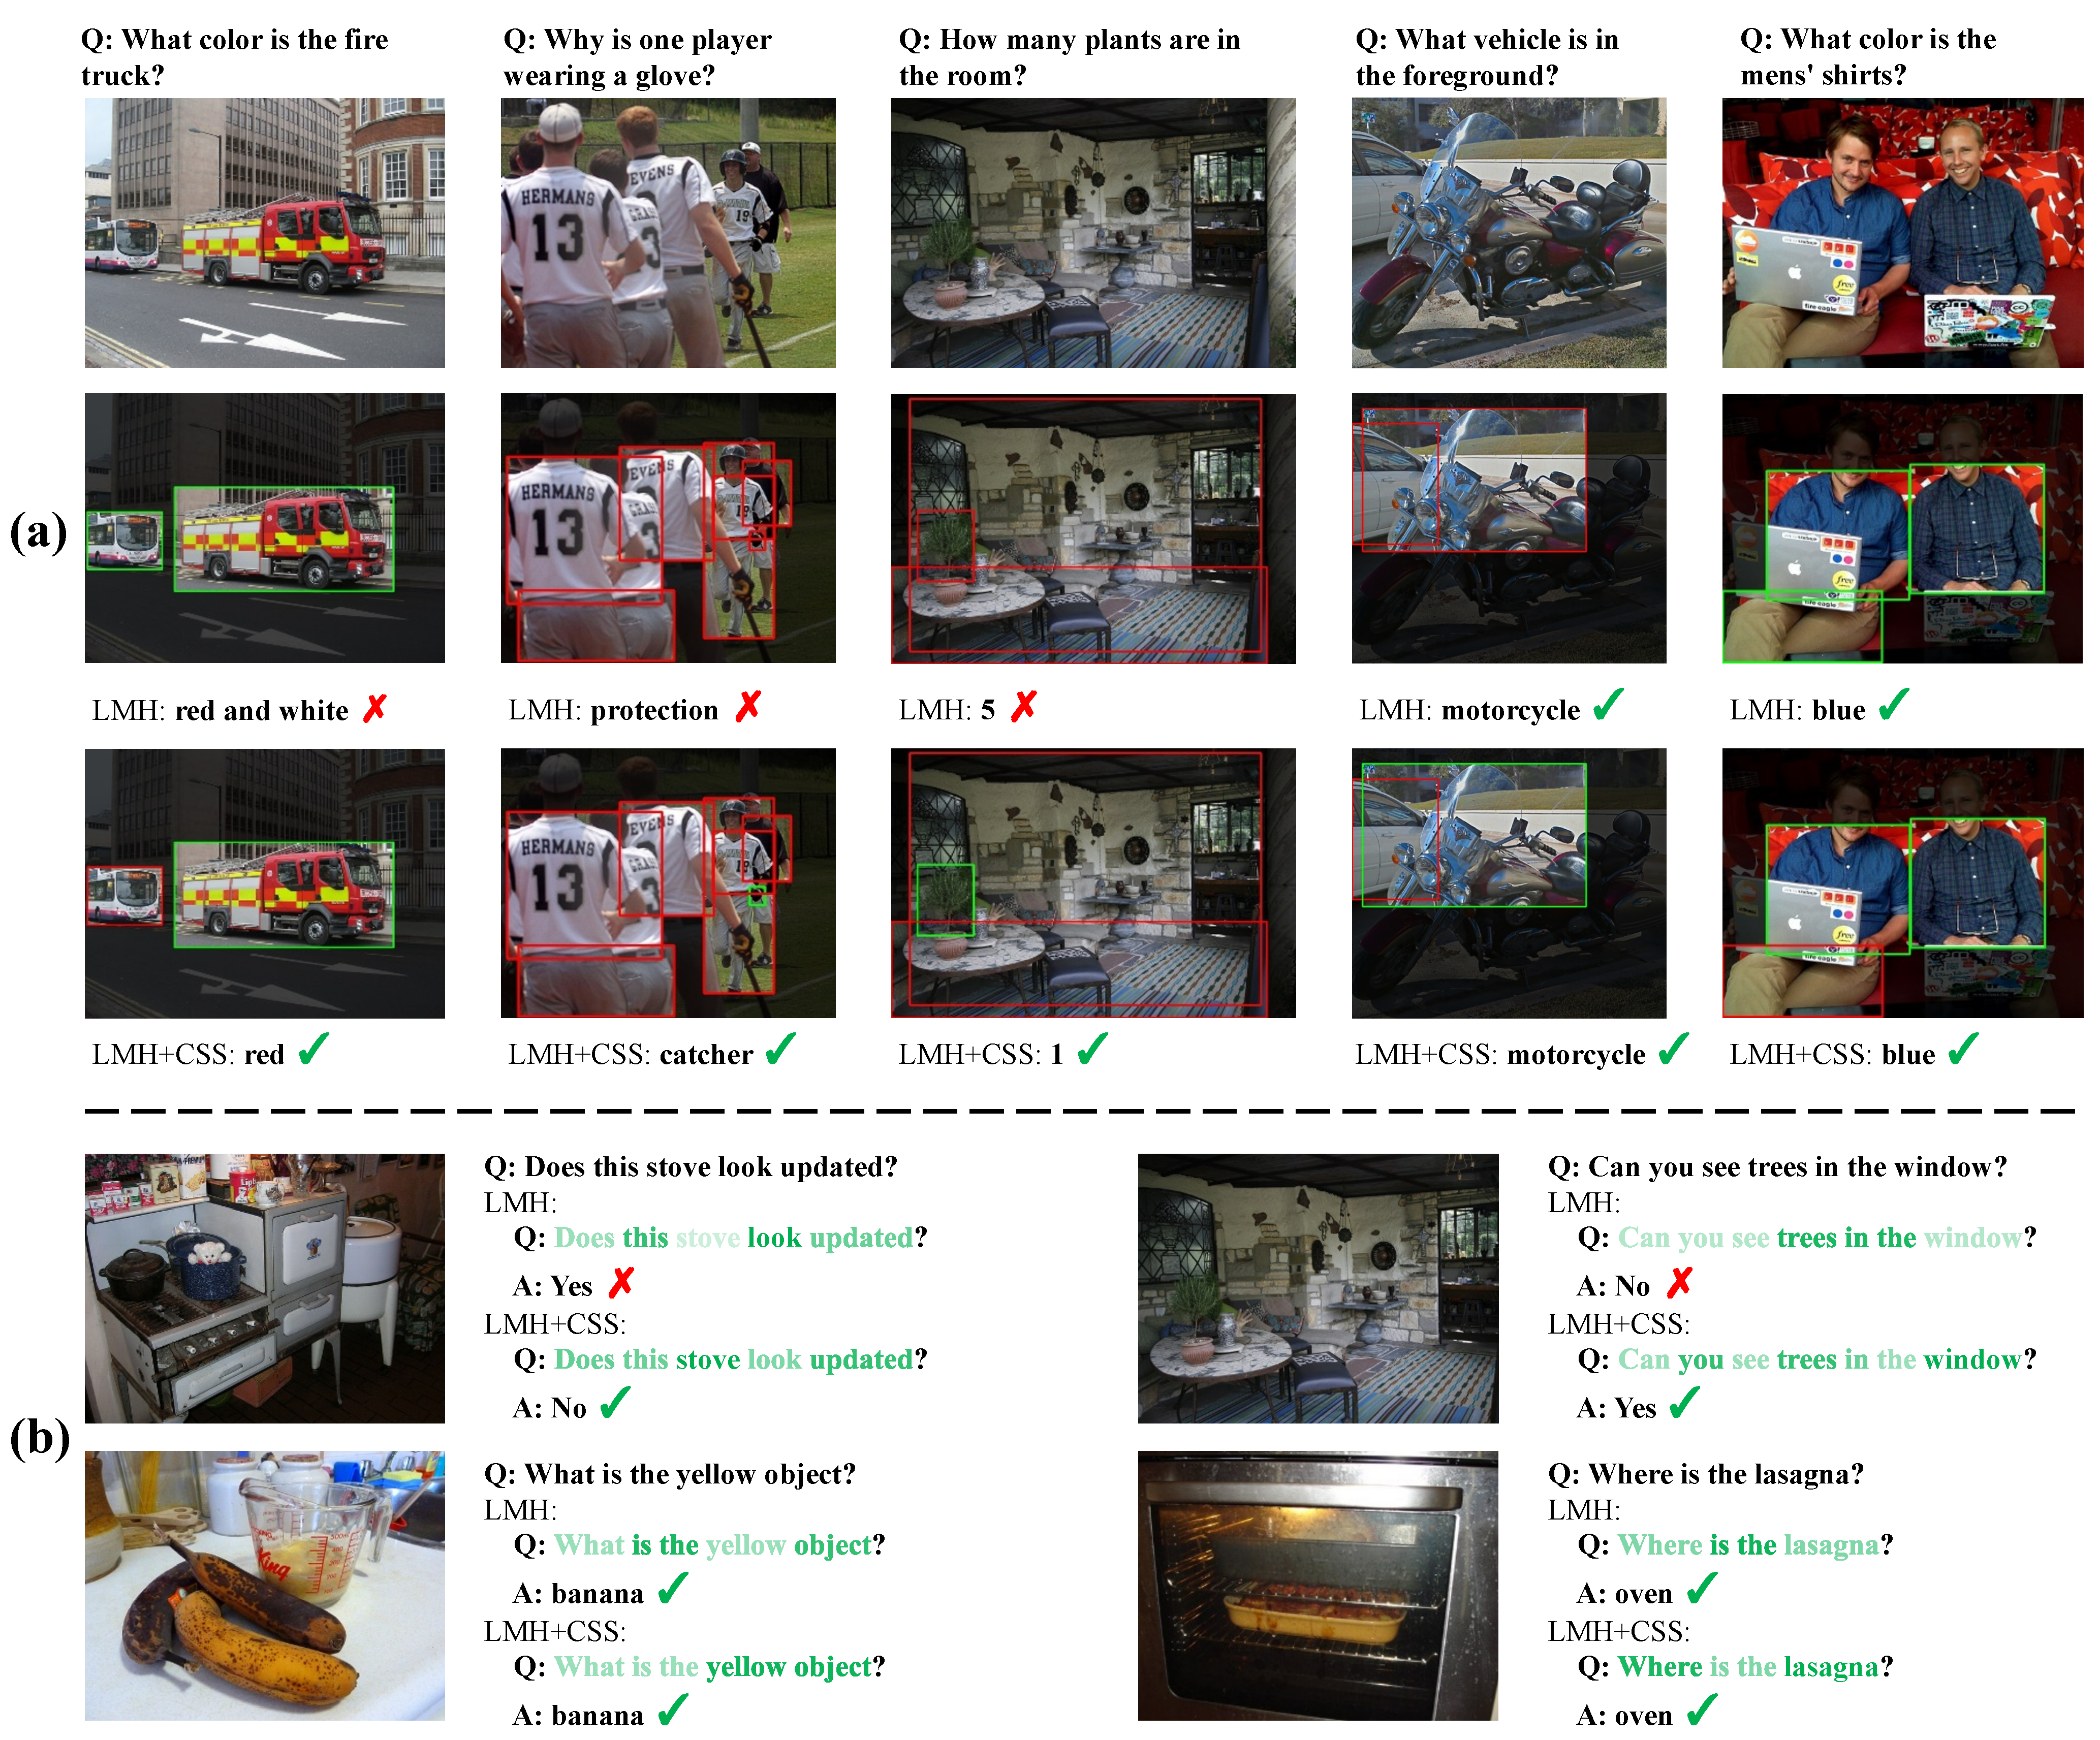
\includegraphics[width=\linewidth]{chapter7/res/visualization.pdf}
    \caption{可视化结果}
    \label{ch7:fig:visualization}
\end{figure}


\section{本章小结}
本章,我们提出了一种全新的反事实样本生成机制(Counterfactual Samples Synthesizing, CSS)。CSS不仅仅可以提升模型的视觉可解释性和文本敏感性,同时可以提升不同模型的视觉问答性能。CSS通过遮盖重要的物体和单词,迫使模型更加关注被遮盖的区域。更进一步,1)我们可以将CSS扩展到其他的多模态任务,减缓文本偏置的影响;2)或者设计一个VQA的骨干网络,使得模型更加有利于CSS的训练。